\documentclass[journal]{IEEEtran}
\usepackage{graphicx}
\usepackage[utf8]{inputenc}
\usepackage{float}
\ifCLASSINFOpdf
\else
\fi
\hyphenation{op-tical net-works semi-conduc-tor}
\begin{document}
\title{SHA-256 PAPER}
\author{Eduard~Torres~Chaves~\IEEEmembership{}
        and~Juan~José~Solano~Quesada~\IEEEmembership{}
\thanks{E. Torres Chaves Computer Engineering student, Instituto Tecnológico de Costa Rica}% <-this % stops a space
\thanks{J.J. Solano Computer Engineering student, Instituto Tecnológico de Costa Rica}% <-this % stops a space
\thanks{}}
\maketitle
\begin{abstract}
hay que hacerlo al mfinal 

\end{abstract}
\begin{IEEEkeywords}
aun no se 
\end{IEEEkeywords}
\IEEEpeerreviewmaketitle

\section{Introduction}
In this paper we will talk about the study and experimentation of the SHA-256 hash function, is important to know that SHA-256 isn't an encryption algorithm, it is a ‘one-way’ cryptographic function.\ SHA-256 is a member of the SHA-2 family, which was designed by the United States National Security Agency (NSA).\\ It's one of the successor hash functions to SHA-1, but is not much complex.The uses of SHA-256 goes from hash tables, integrity verification, challenge handshake authentication to digital signatures, etc.\\ 
The fact of being a cryptographic hash functions is their collision resistance: nobody should be able to find two different input values that result in the same hash output.\\
SHA-256 creates an 256-bit key (from there comes the name), that make it perfect partner-function for AES(Advanced Encryption Standard) and other's alike.
\section{Methodology}
The chosen model is the qualitative one, because it allows us to use experimentation to obtain the necessary data to reach conclusions about the function, we will make distinct experiments around the Java code of the SHA-256 function, once we finish the tests, we will compare then to know the trend of the function with different sizes of input text and the time spent in "digesting" them.\\heil 
The string list used in the experiments is:
[ "abc","test", "one after one", "Heil Hitler", "today is gonna be a beautiful day", "I don't think you trust\ In my self righteous suicide\ I cry when angels deserve to die!"].\\
In the figure 1, is the result of a python code that counts the number of characters which has each string in the previous list, the difference in numbers of characters is important for the test diversity(the presence of uppercase and lowercase letters should not affect the digesting time). \\
 Next is the Java code (figure 2) that is used in the test realization, the code has a string which is digested and comes out in a byte vector, which is manipulated to be transformed into a readable string.
\begin{figure}[h] 
	\centering 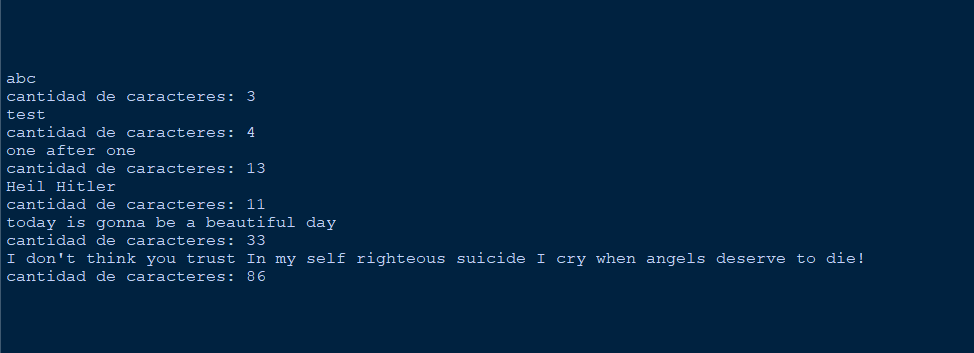
\includegraphics[width=.70\columnwidth]{CantidadDeCaracteres.png}
	\caption{
		\label{fig:samplesetup}
		Result of the character counter in Python
	}
\end{figure}
\begin{figure}[h] 
	\centering 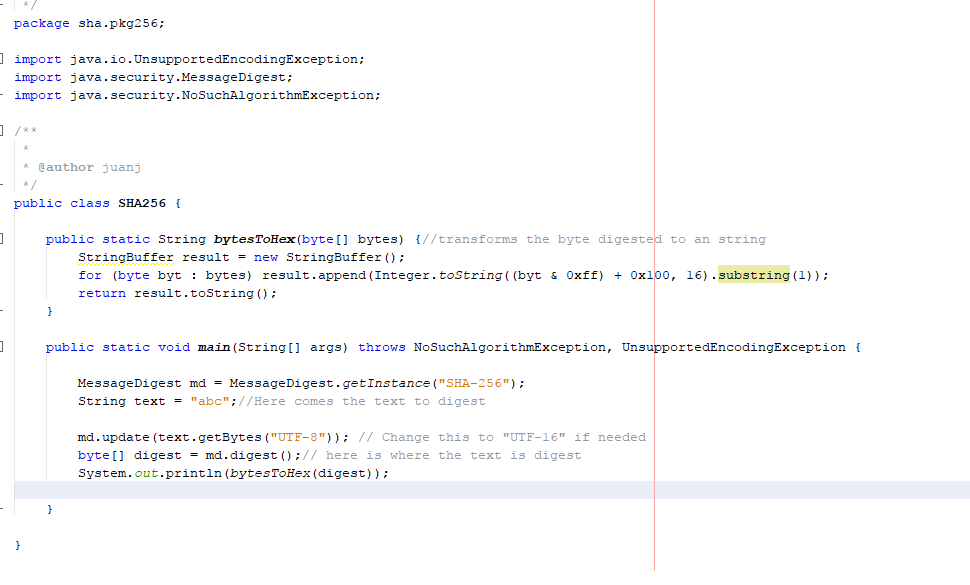
\includegraphics[width=.70\columnwidth]{Sha-256Code.png}
	\caption{
		\label{fig:samplesetup}
		SHA-256 Java Code 
	}
\end{figure}
\section{Experimentation}

\end{document}